Ein weiteres, nicht minder bedeutendes Thema befasst sich mit der
Zeitumrechnung. Dabei bildet die Sonne, angelehnt an das heliozentrische
Weltbild (die Erde dreht sich um die Sonne), den gemeinsamen Bezugspunkt für
Erde und Mars.

Die Erde bewegt sich mit einer Geschwindigkeit von $27$ $\frac{km}{h}$ auf einer
elliptischen aber fast kreisförmigen Umlaufbahn um die Sonne (siehe Bild
\ref{fig:marsEarthOrbit}).

\begin{figure}[H]
	\centering
	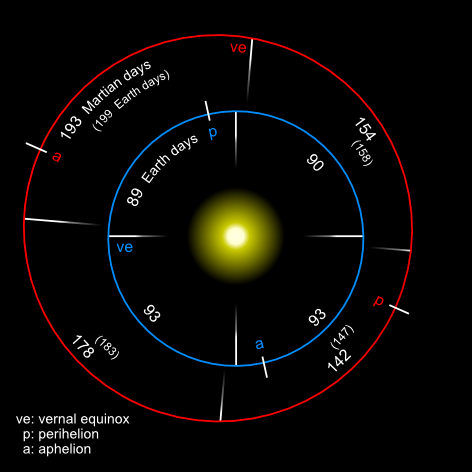
\includegraphics[scale=.5]{Mars_earth_orbit.png}
	\label{fig:marsEarthOrbit}
\end{figure}

Die Drehrichtung ist rechtläufig. Das heißt die Bewegung erfolgt entgegen dem
Uhrzeigersinn um die Sonne. Mit gleichem Drehsinn erfolgt eine Eigenrotation
der Erde. Diese wird als sidierischer Tage bezeichnet und ist nach $23$ Stunden
und $56$ Minuten vollzogen. Die fehlenden $4$ Minuten, zu dem uns geläufigen
$24$ Stunden-Tag (Sonnentag), lässt sich durch äußere Einwirkungen, wie die
Anziehungskraft der Sonne erklären. Von dieser Betrachtung ausgehend, benötigt
die Erde für einen einmaligen Umlauf um die Sonne $365.2424$ Sonnentage, was
einem Erdenjahr (tropisches Jahr) oder einem terrianischen Jahr entspricht. 

Die selben Vorraussetzungen gelten ebenfalls für den Mars. Das Bild zeigt
\ref{fig:marsEarthOrbit} für den Mars eine viel elliptischere Bahn auf. Dies hat
eine Verschiebung der Tages und Jahreszeiten zur Folge. Somit ist auf dem Mars
ein Sonnentag exakt $24$ Stunden, $39$ Minuten und $35.24$ Sekunden lang und
wird "Sol" (Sol, engl. solar day) genannt. Nach $686.9710$ Erd-Sonnentagen bzw.
$669$ Sol hat der Mars die Sonne einmal vollständig umkreist. Um eine Beziehung
und somit eine Umrechnung der Zeiten zwischen Planeten vorzunehmen, muss die
Einteilung der Monate und Jahreszeiten aus Sicht der Sonne, wie eingangs
erwähnt, vorgenommen werden. 

Im Weiteren soll eine Möglichkeit zur Umrechnung der Erdzeit auf Marszeit, nach
Robert Zubrin,  welcher auch den Begriff "Sol" für einen Marstag prägte,
vorgestellt werden. Die nachfolgende Abbildung zeigt den von Zubrin entwickelten
Marskalender (Bild \ref{fig:marsEarthCalendar} links) im Vergleich zu dem uns
bekannten gregorianischen Kalender. Die Monate sind hierbei zur einheitlichen
Bestimmung in Form der lat. Namen der Tierkreiszeichen welche sie zu jener Zeit
von der Sonne aus gesehen durchziehen.

\begin{figure}[H]
	\centering
	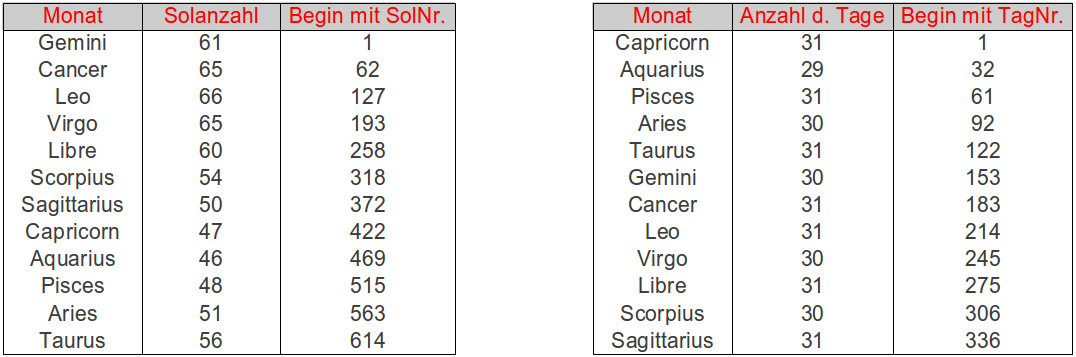
\includegraphics[width=\textwidth]{marsEarthCalendar.png}
	\label{fig:marsEarthCalendar}
\end{figure}

Bei der Umrechnung zwischen diesen beiden Kalendern, bezog sich Zubrin auf das
Jahr $1965$. Dort fielen der Beginn des Erdenjahres ($1.$ Januar), sowie der
Beginn des Marsjahres ($1.$ Gemini) aufeinander. Daraus ergab sich der
nachfolgende Ansatz:

\begin{equation}
	Marsjahr \quad = \quad (\frac{8}{15}) \quad * \quad (Erdjahr - 1961) \quad + \quad 1
	\label{eq:marsYear}
\end{equation}

Das Erdenjahr folgt einer dezimalen Darstellung und setzt sich wie in Formel
\ref{eq:earthYear} zusammen. Zum Tragen kommen hierbei das aktuelle Jahr, sowie
die numerischen Angaben von Tag ($numAktTag$) und Monat ($numAktMonat$) des zu
umrechnenden Datums. Dies wird ins Verhältnis zur Gesamtanzahl der Tage in einem
Jahr gesetzt.

\begin{equation}
	Erdjahr \quad = \quad aktuelleJahr + \frac{ (numAktMonat - 1) * 30.4 + (numAktTag - 1) }{365}
	\label{eq:earthYear}
\end{equation}

Diese soll am Beispiel der Marslandung der Sonde "Curiosity", am $6.$ August
$2012$, verdeutlicht werden.

Aus Gleichung \ref{eq:earthYear} wird zunächst das dezimale Erdjahr berechnet.
Es ergibt sich:

\begin{eqnarray}
	Erdjahr \quad & = & \quad 2012 + \frac{ (8-1) * 30.4 + (6-1) }{365} \notag\\
	Erdjahr \quad & = & \quad 2012 + 0.59 \notag\\
	Erdjahr \quad & = & \quad 2012.59
\end{eqnarray}

In die Gleichung \ref{eq:marsYear} eingesetzt

\begin{eqnarray}
	Marsjahr \quad & = & \quad (\frac{8}{15}) * (2012.59 - 1961) + 1 \notag\\
	Marsjahr \quad & = & \quad 28.51
\end{eqnarray}

ergibt das Marsjahr $28$. Der jeweilige Tag und Monat des Jahres wird
schlussendlich durch die Gleichung \ref{eq:MarsMonthSol} und die Tabelle
\ref{fig:marsEarthCalendar} bestimmt.

\begin{eqnarray}
	Marstag \quad & = & \quad \#MarstageImJahr * restMarsjahr \\
	Marstag \quad & = & \quad 666 * 0.51 \notag\\
	Marstag \quad & = & \quad 340 Sol \notag
	\label{eq:MarsMonthSol}
\end{eqnarray}

Damit ist die Marssonde "Curiosity"' am $22.$ Sol im Sternbild Scorpius des 
Marsjahres $28$ auf dem Mars gelandet.

Jedoch weist Zubrin's Ansatz einige Fehler auf, die auf den ersten Blick zwar
nichtig erscheinen, jedoch auf weite Sicht starke Verschiebungen der Zeiten zur
Folge haben. Die Annahme, ein Erdenjahr sei immer $365$ Tage lang (siehe Formel
\ref{eq:earthYear}), kann nicht verallgemeinert werden. Vielmehr muss von einem
Mittel ausgegangen werden, da die Länge eines Erdenjahres aufgrund der sich
wechselnden Abstände zur Sonne variiert. Hier wird das sogenannte Tropische Jahr
herangezogen, welches $365.2424$ Tage lang ist. Davon ausgehend, ist eine
Korrektur des in der Formel \ref{eq:earthYear} angenommenen Verhältnisses von
Mars- zu Erdenjahr (erster Term) auf $\frac{7.97}{15}$ notwendig (Nachweis ab
Formel \ref{eq:errorKorrektur}).

\begin{eqnarray}
	\frac{MarsJahr}{ErdJahr} \quad & = & \quad \frac{686.9710 \ Tage}{365.2424 \ Tage}
	\\
	\label{eq:errorKorrektur}  
	\frac{MarsJahr}{ErdJahr} \quad & = & \quad 1.88 \notag\\
	\notag\\
	x \quad & = & \quad \frac{15}{1.88} \notag\\
	x \quad & = & \quad 7.97 \notag
\end{eqnarray}

Damit würde sich das Landungsdatum der Marssonde auf den $16.$ Sol im Sternbild
Libre verschieben. Nach nur knapp $50$ Jahres der Zeitrechnung Mars stellt sich
schon eine Verschiebung von $66$ Sol ein. Dies zeigt dass eine exakte Umrechnung
der Daten von nöten ist, um eine langfristige Aussage über das Datum und die
Zeit auf dem Mars zu machen.
